\textcolor{lila}{Här presenteras huvuddragen av varje problem samt den tillhörande informationen. Notera att allt runtomkring själva problemet enbart är förslag, och att varje lärare kan anpassa genomförandet efter hur hen tror att det blir bäst i en specifik klass. Problemen i avsnitt \ref{sec:Fermi} till och med \ref{sec:Sortera} är allmänna problem som inte kräver några speciella förkunskaper från läraren, förutom det som skickas med som kompletterande information. Övriga problem baseras på programmering, och det är då lättare för läraren att hjälpa till med koden om denne kan programmera. Notera dock att det är problemlösningen som står i centrum, och inte kodens specifika syntax. Lärarna får även själva välja vilket programmeringsspråk som ska användas, men som vägledning skickas ett lösningsförslag skrivet i Java. Alla problemen finns även i sin fullständiga form i appendix~\ref{appendix:Problem}.}

\subsubsection{Fermiproblem}
    \label{sec:Fermi}
 
    \textcolor{lila}{Målet med detta problem är att eleverna ska få träna på att göra uppskattningar, samt att bryta ner ett problem i mindre delar.}
    
    \textcolor{lila}{Som inledning presenteras vad ett \textsl{fermiproblem} är. Det innebär att man, i fall där ett specifikt värde inte är svårt alternativt omöjligt att mäta, bryter ner problemet i många små delar och uppskattar varje del för sig. På så sätt kan man uppskatta lösningen på frågor som vid första anblick kan verka omöjliga. För att illustrera detta visas även ett exempel på ett fermiproblem, samt exempel på hur man kan dela upp det i minde delar.}

    \textcolor{lila}{Eleverna får en lista med olika fermiproblem att välja mellan, och ska arbeta i grupper om 2. Först ska de gissa på svaret, och sedan beräkna det genom att dela upp i delar som man kan uppskatta. Därefter får de i mindre grupper presentera och diskutera sitt arbete. Slutligen diskuteras i helklass om resultaten kändes rimliga, hur genomförandet gick, ifall lösningsmetoden är användbar samt varför den fungerar så bra som den gör. För den sista frågan ger vi även lärararen svaret, det vill säga att det fungerar eftersom man ibland överskattar och ibland underskattar de mindre delarna, vilket gör att det slutgiltiga resultatet ofta blir en mycket bra uppskattning.}

\subsubsection{Flygplan}
    \label{sec:Flygplan}
    
    \textcolor{lila}{Detta  problem syftar till att träna eleverna på ett undersökande arbetssätt där inte alla påverkande faktorer är givna, utan måste resoneras fram av eleverna. Den leder också fram till ett ekvationssystem, vilket ger ett exempel på när dessa är användbara.}
    
    \textcolor{lila}{En Sverigekarta med utmarkerade flygplatser och flygrutter presenteras för klassen, se figur~\ref{fig:Flygplan}. Detta görs bitvis, med plats för en kort diskussion om vad frågeställningen skulle kunna vara, givet den dittills givna informationen. Med all information given får eleverna i grupper om två arbeta med en specifik sträcka, Visby-Karlstad. På vilka olika sätt kan man ta sig mellan dessa två städer? Vilken sträcka är bäst och vilka faktorer påverkar detta? Därefter specificeras uppgiften ytterligare, genom att de får reda på hur mycket det kostar att åka mellan två olika direkta flygsträckor. De ska nu hitta den \textsl{billigaste} vägen mellan Karlstad och Visby, samt vilken väg som blir billigast om man ska från Karlstad till Stockholm, men sträckan Stockholm-Göteborg är fullbokad. Den avslutande helklassdiskussionen tar bland annat upp vilka faktorer som påverkar bränslekostnaden, vilka faktorer som påverkar biljettpris för en specifik sträcka och ifall det är det totala avståndet eller antalet mellanlandningar som avgör priset för en resa.}
    
    \textcolor{lila}{Under punkten ''Ytterligare information'' diskuteras tankar bakom uppgift och diskussion. Eleverna får själva upptäcka att priset beror på sträckan, men att det också tillkommer ett fast pris för start och landning, vilket speciellt visar sig i att det för sträckan Karlstad-Göteborg blir billigare att flyga en längre sträcka, men med färre mellanlandningar. De får också själva reflektera över ytterligare faktorer som skulle kunna påverka priset, till exempel löner och vinstmarginal.}
    
\subsubsection{Fritt fall}
    \label{sec:FrittFall}
    
    \textcolor{lila}{Tanken med problemet är att eleverna ska få använda derivata utifrån en verklig situation istället för utifrån en färdig formel, samt få en djupare förståelse för vad derivata egentligen är.} 
        
\begin{figure}
    %\centering
    \hspace{0.4cm}
    \begin{subfigure}[b]{0.45\textwidth}
        \centering
        %\hspace{-40pt}
        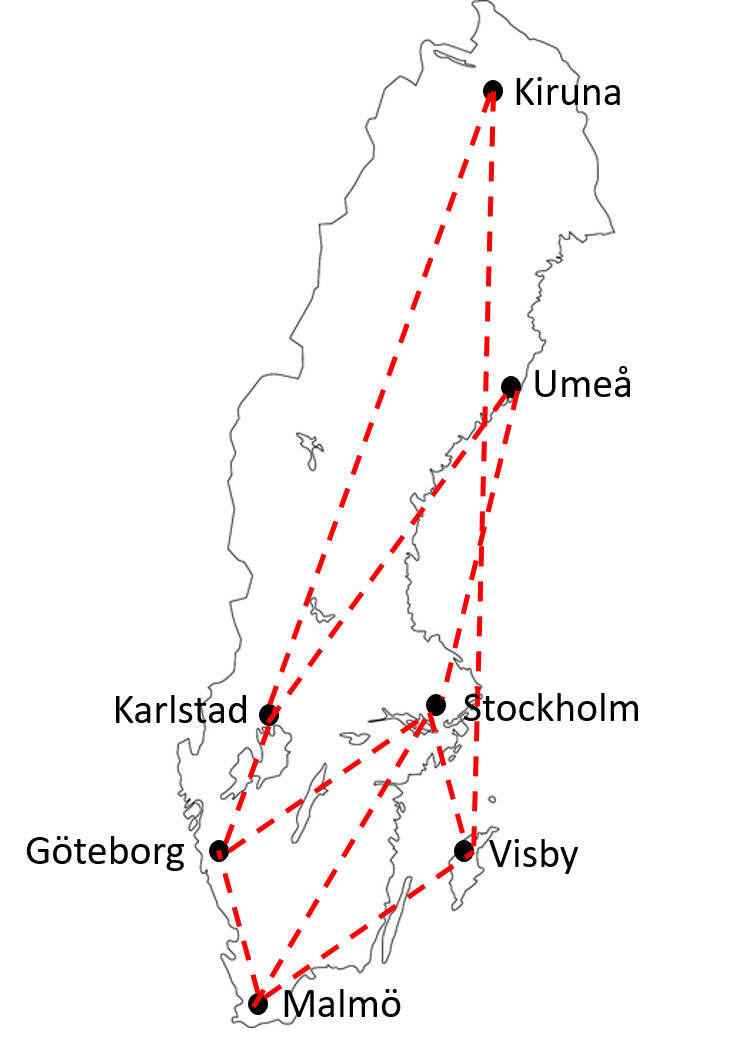
\includegraphics[width=0.9\textwidth]{Figures/Flygplan_rapport.png}
        \caption{\textsl{Sverigekarta med utmarkerade flygplatser och rutter.}}
        \label{fig:Flygplan}
    \end{subfigure}
    \hfill
    \begin{subfigure}[b]{0.45\textwidth}
        \centering
        %\hspace{-40pt}
        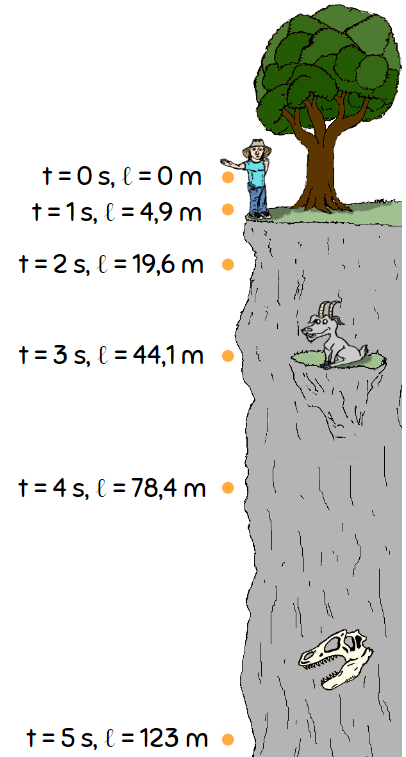
\includegraphics[width=0.7\textwidth]{Figures/FrittFall.PNG}
        \caption{\textsl{Fallande boll med angivna fallsträckor för varje sekund.}}
        \label{fig:FrittFall}
    \end{subfigure}
    \hspace{0.4cm}
    \caption{Figurer tillhörande två av problemen, ''Flygplan'' till höger och ''Fritt fall'' till vänster.}
    \label{fig:three graphs}
\end{figure}
    
    \textcolor{lila}{Som en introduktion till problemet diskuterar man tillsammans i klassen vad en derivata är och hur man kan beräkna den. Därefter presenteras en bild av en fallande boll, med utmarkerade fallsträckor för olika tider, se figur~\ref{fig:FrittFall}. Frågan är nu vad man utifrån detta kan komma fram till om bollens hastighet och acceleration, vilket klassen får arbeta med i grupper om två. Tanken är att man ska konstruera en graf över sträcka som en funktion av tid, och utifrån denna använda en linjal för att rita tangenter längs med grafen och därmed skapa en graf över hastighet som en funktion av tiden. Därefter kan samma procedur genomföras för att rita accelerationen som funktion av tiden. Denna bör, med avvikningar på grund av felkällor, bli konstant och ungefär lika med tyngdaccelerationen, det vill säga ungefär 10. Avslutningsvis diskuteras denna metod med avseende på resultat och noggrannhet.}
    
\subsubsection{Försvåring av en ekvation}
    \label{sec:ekvation}

    \textcolor{lila}{Detta är en mycket fri uppgift med målet att ge eleverna en djupare förståelse för ekvationer och ekvationslösning.}

    \textcolor{lila}{Inledningsvis diskuteras begreppet ekvation, samt hur man löser en ekvation, i helklass. Det viktiga här är att komma fram till att så länge man gör samma sak på båda sidorna om likhetstecknet, och använder prioriteringsreglerna rätt, så får man göra vad som helst. Eleverna får därför två och två arbeta med att ''försvåra'' ekvationen x=2, genom att i flera steg göra en bestämd operation i både vänster- och högerledet. Följande enkla exempel på hur man kan börja presenteras för eleverna som tips på hur man kan börja}
    
        \begin{equation*}
            x=2
        \end{equation*}
        \begin{equation*}
            2x=4 \quad (\cdot2=\cdot2)
        \end{equation*}
        \begin{equation*}
            2x+5=7+2 \quad (+5=+3+2)
        \end{equation*}
    
    \noindent\textcolor{lila}{Varje steg ska även skrivas upp och motiveras enligt ovan. Därefter diskuteras lösningsgången, samt potentiella utvecklingar. Eleverna får också diksutera ifall det finns någon lösning på ekvationen, och hur den i så fall ser ut. De får på så sätt reflektera över att de nu har ''löst en ekvation baklänges'' och att varje ekvation, som kan tyckas se jobbig ut, kan brytas ner i små, enkla steg.}

\subsubsection{Matematisk modell för löpare och bil}
    \label{sec:lopare}
    
    \textcolor{lila}{Detta problem är ursprungligen förklätt som en enklare standarduppgift, men låter därefter eleverna fundera över den matematiska modell de har använt, samt ifall den är rimlig. Målet är att visa fördelar och nackdelar med matematiska modeller, samt införa ett sunt kritiskt tänkande hos eleverna.}
    
    \textcolor{lila}{Inledningsvis får eleverna i par lösa två till synes likartade uppgifter av standardkaraktär. I den ena får de givet hur snabbt det tar att köra en viss sträcka med bil, och ska beräkna hur lång tid ett antal andra sträckor tar att köra. I den andra uppgiften är bilen utbytt mot en löpare, men för övrigt är det samma frågeställning. Vi upplyser här läraren om att vi antar att de flesta elever kommer använda en linjär modell, dvs anta att både bilen och löparen håller samma fart oavsett sträcka. Därefter diskuterar men resultaten i helklass, samt vilka antaganden man har gjort, om de är rimliga och om det skiljer sig mellan bilen och löparen. Som jämförelse får man reda på att den tid som med den linjära modellen fås för den längsta sträckan för löparen är betydligt snabbare än världsrekordet, och man får även verkliga tider för de efterfrågade sträckorna\footnote{Tiderna för löparen som använts är tagna från hur fort Axel, medförfattare i detta arbete, springer dessa sträckor.}. Utifrån detta får eleverna diskutera vilka faktorer som avgör, till exempel att man orkar springa snabbare på kortare sträckor, men också att startsträckan tar upp större delen av tiden.}
    
\subsubsection{Sortera en kortlek}
    \label{sec:Sortera}
    
    \textcolor{WildStrawberry}{
        Kortleken är ett enkelt sätt för en elev att få en god introduktion till hur enkla sorteringsalgoritmer fungerar samt hur man nyttjar sig av dem. }
        
    \textcolor{WildStrawberry}{
        Lektionen kommer innefatta att eleven får en introducerande beskrivning på vad en algoritm är och hur den kan användas. Sedan kommer eleverna få fundera en stund på hur man kan utnyttja algoritmer till att bryta ner större problem till enkla upprepande arbetsflöden. Till uppgiften så kommer kortlekar att tillhandahållas till eleverna som får instruktioner på hur man får interagera med sina kort när man försöker sortera dem, dessa instruktioner efterliknar sättet en dator jämför och byter postition på element i en lista. När eleverna fått experimentera och kommit fram till sina algoritmförslag så skriver dem ner sina instruktioner. De byter instruktioner med en annan grupp och ska kunna sortera sina lekar genom att enbart följa instruktionerna, precis som en dator hade gjort. }
        
    \textcolor{WildStrawberry}{
        Den stora lärdommen i denna uppgift är att eleverna i fråga troligtvis lyckas skapa algoritmer som har givna namn och som faktiskt används i ''den riktiga världen''.  Eleverna kommer få reflektera över vad som gått bra, eller dåligt, och hur man kan göra optimeringar eller fixa problemen (''buggarna'') som uppstod. Ungefär som en riktig programmerare får göra. \todo{:)}}
        
    
\subsubsection{Fibonaccis talsekvens}
    \label{sec:Fib}
    
    \textcolor{WildStrawberry}{
        Fibonaccis talsekvens är mycket klassiskt problem när det kommer till programmering. Det är ofta en startpunkt för rutinerade programmerare som försöker lära sig syntaxen i nya programmeringsspråk (förutsatt att man känner till lösningen). }
        
    \textcolor{WildStrawberry}{
        Undervisningen kommer bestå av att läraren introducerar Fibonaccis talsekvens och hur talföljden utvecklar sig. Efter detta kommer eleverna försöka skapa egna stycken kod som ska skriva ut talföljden. Mer erfarna programmerare uppmuntras till att prova lösa uppgiften med hjälp av rekursion. När väl eleverna provat att lösa uppgiften så kommer en diskussionstund där man bör reflektera på hur det har gått, hur väl sin kod fungerar och vilka optimeringar som man kan göra. Slutligen kan man diskutera och reflektera över hur man kan använda sig av loopar för att lösa problem.}
        
    \textcolor{WildStrawberry}{
        I denna uppgift får får eleven träning i iterativa och rekursiva loopar. Båda vilka är verktyg som programmerare behöver kunna använda sig utav. Lär man sig behärska dessa tekniker så kommer man i sin följd kunna lösa andra problem som har iterativ, eller rekursiv, struktur.}
        
\subsubsection{Personnummer}
    \label{sec:Pnr}
    
    \textcolor{WildStrawberry}{
        }
        
\subsubsection{Primtalsfaktorer}
    \label{sec:Primtal}
    
    \textcolor{WildStrawberry}{
        Att kunna faktorera tal in till primtal är något man kan råka stöta på i sitt liv. Kanske speciellt om man någon gång behöver nyttja sig av eulers phi-sats..... \todo{this is bajs!} }
        
    \textcolor{WildStrawberry}{
        För att introducera detta problem så krävs ingen lång bakgrund, så exempelvis kan läraren skriva upp en mängd siffror som elevernas program ska kunna köra. Sen kommer eleverna, i små grupper om 2 eller 3, försöka skapa program som hanterar alla fallen. Slutligen kommer klassen diskutera hur man hanterat fallen där talen haft fler än 2 primtalsfaktorer, upprepande faktorer och vilka ''fel'' man lyckats fånga med sina program. }
        
    \textcolor{WildStrawberry}{
        Under detta tillfälle så kommer eleven få öva på enkla booleanska uttryck, matematiska operatorer, optimering av kod och eventuella fält eller listor. Det blir en salig blandning av olika moment i programmering och man utsätts för många olika syntax i en och samma uppgift.}